In order to find solutions which matches real life experiments (at least to a certain degree), we need to ensure ourselves that the assumption in our models are sound.
As important is it to check that the machinery handeling the numerical calculation is correctly implemented.
This can be done by code verification.

Quoting \cite{Dudson2016}

\blockquote{
Code verification is a process of checking that the chosen set of partial differential equations is solved correctly and consistently, and is a purely mathematical exercise.
Code verification is not concerned with verifying that the chosen numerical methods are appropriate for the chosen set of equations.
Code verification is also not concerned with testing the ability of a given model to explain experimental observations.
This testing is dealt with in the subsequent validation process.
}

Thus, a code can be verified numerically, but still fail to match the desired features of a real life experiment.
In other words, it would have passed the verification failed the validation.
If the code has succuessfully passed a validation test, but fails a verification test, the success of the validation is questionable.
The success of the validation in this case could have been a mere coincident.

The verification process is throughly discussed in \cite{Oberkampf2010book}, and more condensed for the method of manufactured solution (MMS) in \cite{Salari}.
Note that the verification process can be time consuming, and can be regarded as an artform in itself.
Luckly, a major part of the implemntation has already been verified in the BOUT++ framework using MMS in \cite{Dudson2016}.

After a quick introduction of the concept of truncation errors, the MMS process will be briefly presented in \cref{sec:MMS} before verification of additional implementations in the CELMA code is given in \cref{sec:MES}.

\section{Numerical errors}
%
Our derivative operators are discretized in order for them to operate on a discretized grid.
Doing so introduces an error, which depends on the order of approximation.
To use a concrete example, let us consider the simplest differential equation
%
\begin{align}
    \deri{f(x)}{x} = g(x)
    \label{ver:ode}
\end{align}
%
where $f(x)$ and $g(x)$ are arbitrary functions (not to be confused with the distribution function and a metric element).
We seek to solve \cref{ver:ode} for $f(x)$.

Let us find the simplest approximation of the derivative in an arbitrary grid point $x_0$.
We first Taylor expand $f(x)$ around $x_0$ and evaluate it in $x_0 + h$ (where $h$ is the grid spacing).
This gives
%
\begin{align*}
    f(x_0+h)
    = f(x_0)
    + h \L.\deri{f(x)}{x}\R|_{x=x_0}
    + \L.\frac{h^2}{2}\deri{^2f(x)}{x^2}\R|_{x=x_0}
    + \mathcal{O}(h^3)
\end{align*}
%
Subtraction of $f(x_0)$ and division by $h$ now yields the following approximation of the derivative
%
\begin{align*}
    \frac{f(x_0+h) - f(x_0)}{h}
    =  \L.\deri{f(x)}{x}\R|_{x=x_0}
    + \L.\frac{h}{2}\deri{^2f(x)}{x^2}\R|_{x=x_0}
    + \mathcal{O}(h^2)
\end{align*}
%
Hence, the local truncation error LTE we do in a single point by using this approximation is
%
\begin{align*}
    \|e_{\text{LTE}}\|
    =
    \L\|\frac{f(x_0+h) - f(x_0)}{h} - \L.\deri{f(x)}{x}\R|_{x=x_0}\R\|
    =
    \L\| \L.\frac{h}{2}\deri{^2f(x)}{x^2}\R|_{x=x_0} + \mathcal{O}(h^2)\R\|
\end{align*}
%
In other words it scales with the grid spacing $h$ to the first order.
The global error in some $L$-norm $n$ can be defined as
%
\begin{align*}
    \L\|\ve{e}\R\|_{L_n} =
    \L\|\ve{f}_{\text{true}} - \ve{f}_{\text{numeric}}\R\|_{L_n}
\end{align*}
%
% FIXME: LTE and global error
where $\ve{f}_{\text{true}}$ is an array of the analytic solution in each grid point, and $\ve{f}_{\text{numeric}}$ is an array of the solution obtained numerically.
From linear PDE theory we have that the global error should converge to the LTE order if the scheme is consistent (the LTE $\to 0$ as $h\to 0$) and numerically stable%
\footnote{Note that the definition of stability depends on the context, see \cite{Leveque2007book} for more details.}.
%
If convergence is observed, the implementation is verified.

\section{Method of Manufactured Solution}
\label{sec:MMS}
For most PDEs, the true solution $\ve{f}_{\text{true}}$ is not known in advance.
Sometimes a solution can be found in some special limits.
If convergence is found for these special cases, the code is not generally verified.
There could still be implementation mistakes (not discoverable in the limiting cases) which could have dire consequences when a more general solution is sought numerically.
One way to get around the problem is to manufacture a solution.

Assume that we have a set of nonlinear spatio-temporal PDEs we would like to solve for.
Let us call the variables evolved in time for $\ve{f}=\{\ve{u}_e, \ve{u}_i, n, \Om^D, T_e, \ldots\}$.
If there are no mixed spatial and temporal variables, we can write the set of nonlinear PDEs as
%
\begin{align}
  \parti{\ve{f}}{t} = F(\ve{f}) \RA \parti{\ve{f}}{t} - F(\ve{f}) = \ve{0}
  \label{ver:setOfPDE}
\end{align}
%
where $F(\cdot)$ is a nonlinear operator which contains the discretized spatial differential operators.
As stated above, we do not know a priori which $\ve{f}$ which satisfies \cref{ver:setOfPDE}.
Therefore we manufacture a set of functions $\ve{f}_M$ which does not satisfy \cref{ver:setOfPDE}, but rather
%
\begin{align*}
    \parti{\ve{f}_M}{t} - F(\ve{f}_M) = \ve{S}
\end{align*}
%
Note that $\ve{f}_M$ is an exact analytical solution of $\parti{\ve{f}}{t} = F(\ve{f}) + \ve{S}$.
We can therefore solve numerically $\parti{\ve{f}}{t} = F(\ve{f}) + \ve{S}$ for $\ve{f}$, and find the global error (for each variable $\ve{u}_e, \ve{u}_i, n, \Om^D, T_e, \ldots$ by
%
\begin{align*}
    \L\|\ve{e}\R\|_{L_n} =
    \L\|\ve{f}_{M} - \ve{f}_{\text{numeric}}\R\|_{L_n}
\end{align*}
%
One can now test if the global error show the expected order of convergence.
Note that $\ve{f}_M$ and the coefficients in the various terms in the PDEs does not need to be physical, but that in order to test all terms in this set of equations, the parameters of the simulation should be chosen so that the magnitude of each term are of a similar order of magnitude.

\section{Method of Exact Solution}
\label{sec:MES}
%

Since there are implementations in this thesis which is not covered by the BOUT++ framework (see \cref{chap:additionalImplementation} for details), these implementation should be verified as well.
All of these implementations are either differentiation operators, extrapolations or integration operators where an exact analytic solution can be found.
Hence, one can use the approach of method of exact solutions (MES) to verify these operations, and there will be no need for manufacturing a solution.

Although it is simpler to perform MES than MMS, there are certain points one should be aware of.
Especially since we are dealing with a periodic domain with a singularity in the center.
Let us now call the function we are operating on with a discretized operator $D$ for $f(\rho,\theta,z)$.
Hence, the source $S$ is given by $D[f(\rho,\theta,z)]=S$, where $S$.
If we are to take derivatives in the $\rho$ direction, we must take care that
%
\vspace{0.5cm}
\begin{enumerate}[noitemsep,nolistsep]
    \item $f(\rho,\theta,z)$ must be of $\mathcal{C}^\infty$ along $\rho$, particularly at \item $f(\rho=0,\theta,z)$.%
    \begin{itemize}[noitemsep,nolistsep]
            \item This implies that the function must also be single valued in $f(\rho=0,\theta,z)$.
            \item Even though the coordinate system have a singularity in $f(\rho=0,\theta,z)$, the function may be continuous in a different coordinate system.
    \end{itemize}
  \item Boundary conditions in $\rho$ must be satisfied.
\end{enumerate}
\vspace{0.5cm}
%
If we are to take derivatives in the $\theta$ direction, we must take care that
%
\vspace{0.5cm}
\begin{enumerate}[noitemsep,nolistsep]
    \item $f(\rho,\theta,z)$ must be of $\mathcal{C}^\infty$ along $\theta$, particularly at $f(\rho,\theta=0,z)$ and $f(\rho,\theta=2\pi,z)$%
    \begin{itemize}[noitemsep,nolistsep]
            \item This implies that the function must also be periodic
    \end{itemize}
\end{enumerate}
\vspace{0.5cm}
%
Note that there are functions not fulfilling all the criteria that can give convergence.

\subsection{Derivative operators}
\label{sec:derOp}
%
We will in this section use the following notation, which is consistent with BOUT++ notation (see \cref{foot:BOUT++coord} in \cref{sec:clebschAlign})
%
\begin{itemize}[noitemsep]
    \item \texttt{DDX(f)} for the second order discretization of $\partial_\rho f$.
    \item \texttt{D2DX2(f)} for the second order discretization of $\partial^2_\rho f$.
    \item \texttt{DDZ(f)} for the spectral discretization of $\partial_\theta f$.
    \item \texttt{D2DZ2(f)} for the spectral discretization of $\partial^2_\theta f$.
\end{itemize}
%
A function which satisfies most of the criteria in \cref{sec:MES} is
%
\begin{align*}
    f(\rho, \theta, z)
    =& \sin\L(
        \frac{1}{\sqrt{2}}\rho[\cos(\theta)+\sin(\theta)]\frac{2\pi}{2L_\rho}
          \R)
      \\&
      \exp\L(
        -\frac{1}{2w^2}
            \L[\rho^2 + \rho_0^2 - 2\rho\rho_0(\cos[\theta - \theta_0])\R]
          \R)
      \\&
        \L(\frac{\rho\cos[\theta]+L_\rho}{2L_\rho}\R)^2,
        \numberthis
        \label{eq:MESf1}
\end{align*}
%
where
%
\begin{align*}
    &L_\rho = 30&
    &\text{
        Cylinder radius
    }&
    \\
    &w = \frac{4}{5}L_\rho&
    &\text{
        Width of Gaussian
    }&
    \\
    &\rho_0 = \frac{3}{10}L_\rho&
    &
    \rho
    \text{
        - coordinate for center of Gaussian
    }&
    \\
    &\theta_0 = \frac{5\pi}{4}&
    &
    \theta
    \text{
        - coordinate for center of Gaussian
    }&
\end{align*}
%
The function is depicted in \cref{fig:typicalMES}, and has the advantage that it is not symmetric across the axis.
However, it is not $\mathcal{C}^\infty$ in $\rho=0$, as the first derivative of the function (with respect to $\rho$) is multivalued there.
As a consequence it is found that for example \texttt{DDX(DDX(f))} diverges rather than converges when applying MES to \cref{eq:MESf1}%
%
\footnote{The ghost points are re-calculated after using the first operation on $f$.}
\footnote{Note that convergence is found for \cref{eq:MESf1} when using \texttt{D2DX2(f)}, and that convergence for \texttt{DDX(DDX(f))} is found using functions which are of $\mathcal{C}^\infty$, but which are not symmetric.\label{foot:DDXDDX}}
%
\begin{figure}[t!]
    \centering
    \begin{subfigure}[t]{0.45\textwidth}
        \centering
        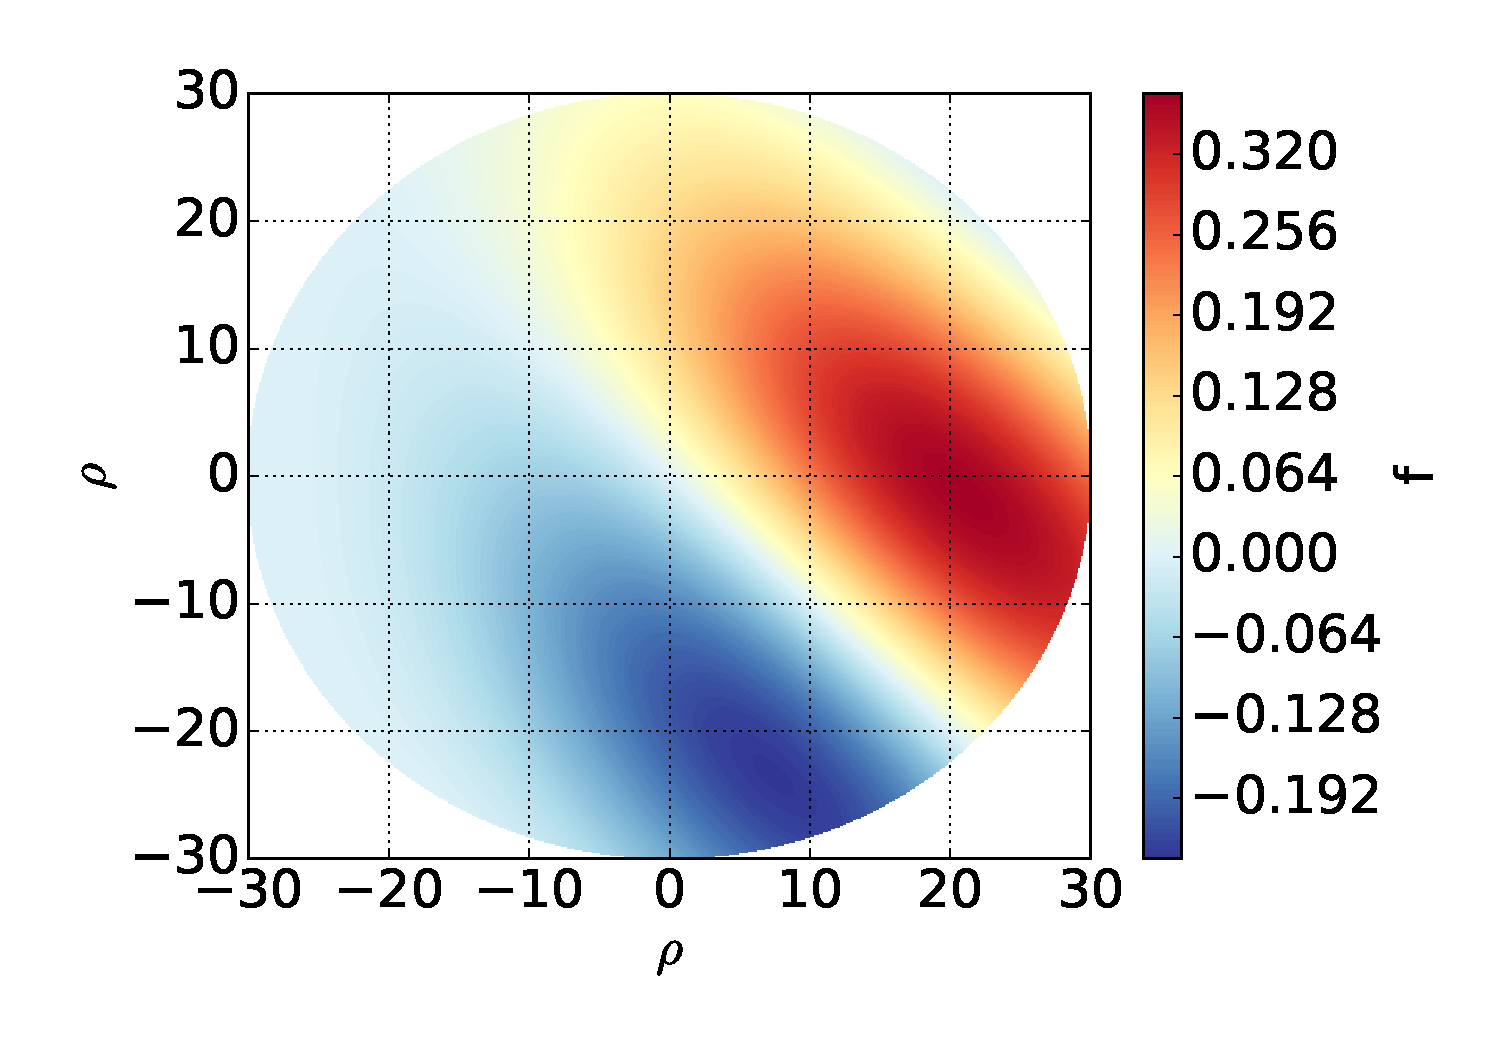
\includegraphics[width=1.0\textwidth]{fig/f}
        \caption{Vizualisation of \cref{eq:MESf1}}
        \label{fig:typicalMES}
    \end{subfigure}%
    ~
    \begin{subfigure}[t]{0.45\textwidth}
        \centering
        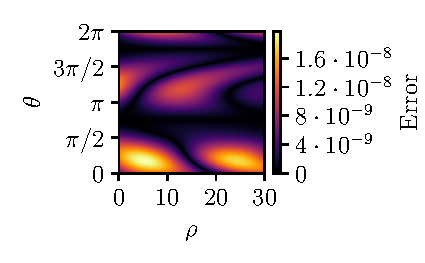
\includegraphics[width=1.0\textwidth]{fig/err}
        \caption{Errors of \texttt{DDX(f)}, where $f$ is given in \cref{eq:MESf1}}
        \label{fig:errorsMES}
    \end{subfigure}
    ~
    \begin{subfigure}[t]{0.45\textwidth}
        \centering
        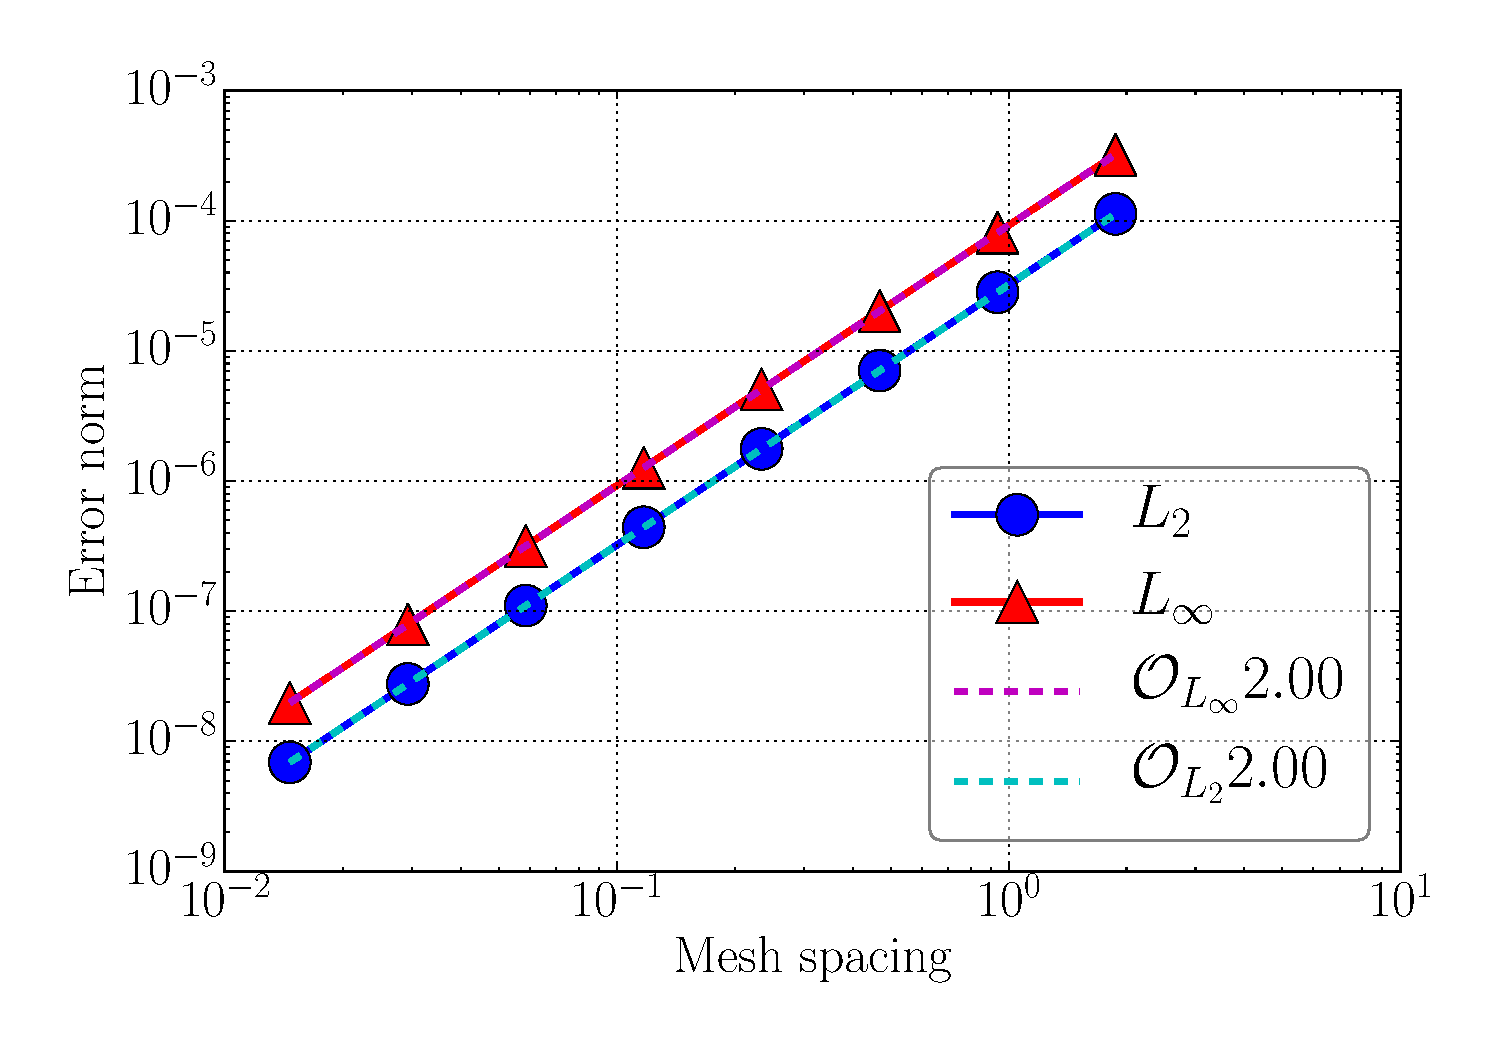
\includegraphics[width=1.0\textwidth]{fig/conv}
        \caption{Convergence rate of \texttt{DDX(f)}, where $f$ is given in \cref{eq:MESf1}}
    \end{subfigure}
    \caption{An example of functions and errors found when using MES.}
\end{figure}

\subsubsection{Single operators}
\label{sec:singleOp}
%
In order to check that the singularity is correctly implemented, we can check that \texttt{DDX(f)} is giving the expected order of convergence on \cref{eq:MESf1} as this is not symmetric.
The error of the operation for $2^{11}$ points is shown in \cref{fig:errorsMES}.
It is important to notice that the error is not dominating at one particular point, but is spread out over domain.
If the inner ghost point were incorrectly implemented, this would be detected by a localized high error around $\rho=0$, and it is expected that the correct order of convergence would not be found.
In addition, we would like to check the convergence of \texttt{D2DX2}, \texttt{DDZ} and \texttt{D2DZ2} as these are used in the $\div\L(g[\grad f]\R)$ operator, and in the $\ve{u}_E^2$ advection of $n$.
The results are given in \cref{tb:MESResults}.
We note that the derivatives in the $\rho$ direction gives the expected second order convergence.
We also see that although the derivatives in the $\theta$ direction seems not to be converging, the errors are quite small.
This is because machine precision is quickly reached.
That is, the loss of precision due to subtraction of two almost equal quantities becomes larger than the error from the discretization itself.
The behavior is depicted in \cref{fig:divDDZ}.
%
\begin{figure}[htb]
    \centering
    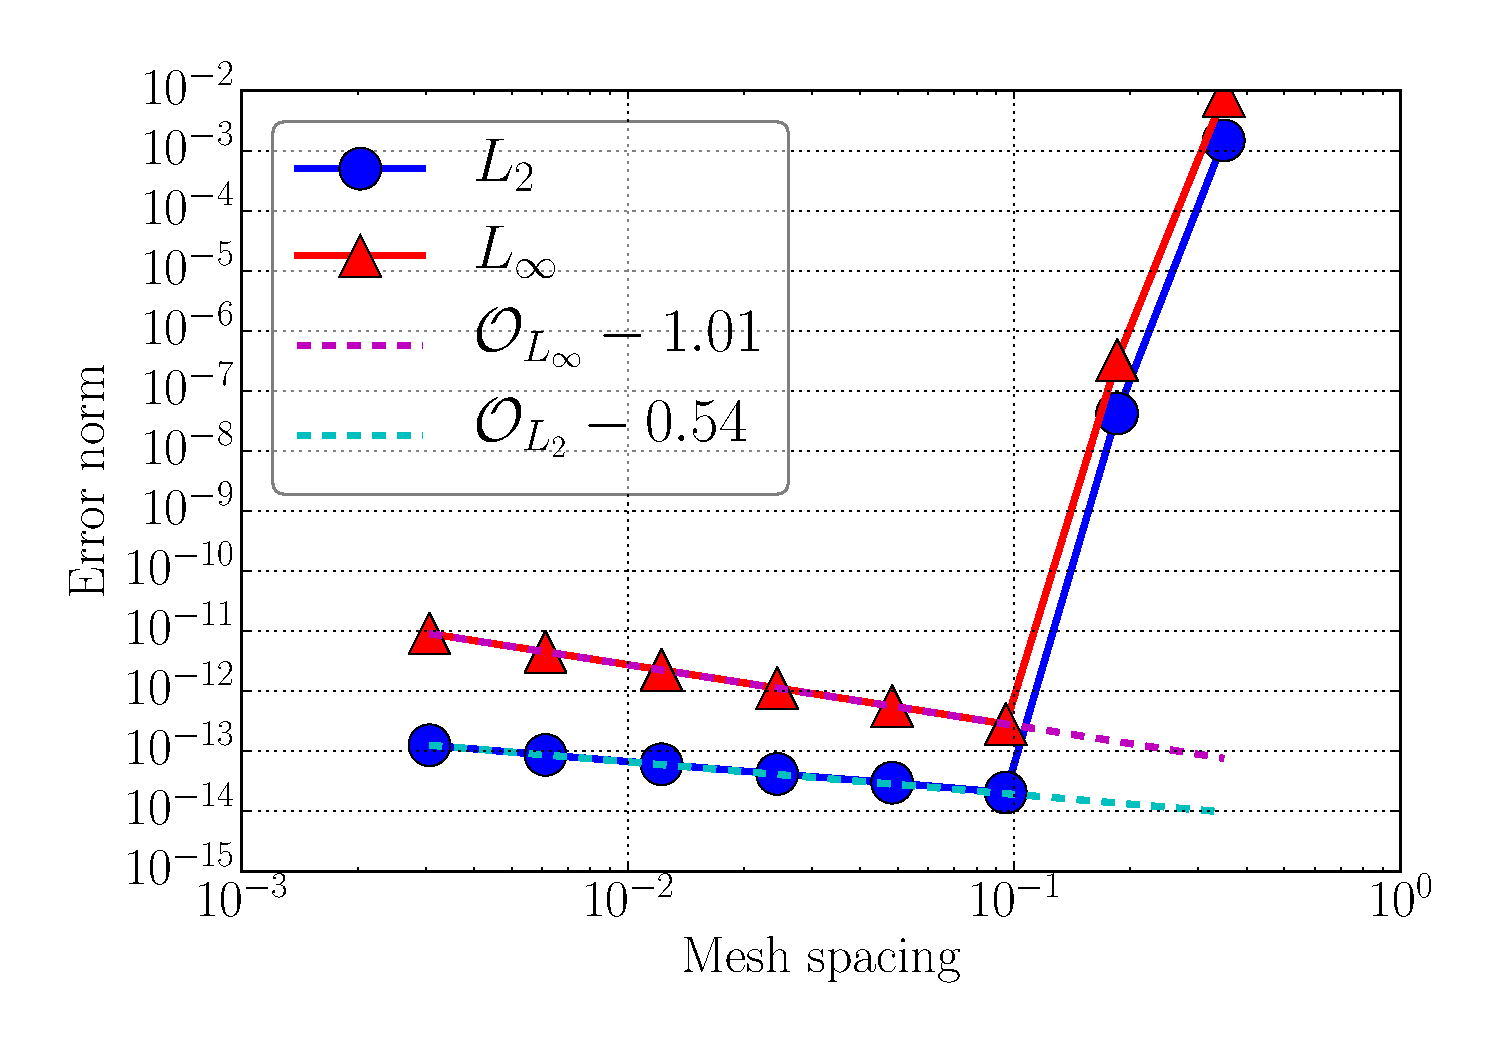
\includegraphics[width=0.5\textwidth]{fig/divDDZ}
    \caption{\textit{
            Divergence due to loss of precision of the operator \texttt{DDZ(f)}.
        }}
    \label{fig:divDDZ}
\end{figure}
%
We therefore consider the schemes up until this point for convergent.

Finally, we will point out an important caveat.
Several operators used in the CELMA code can be written as $\rho^{-n}\partial_\rho f$, and care must be taken as the division by $\rho$ can appear to break the convergence.
In the case of $\frac{\texttt{DDX}(f)}{\rho}$, the loss of expected convergence rate can be explained by looking at the finite difference stencil.
We have that%
%
\footnote{
Found by Taylor expanding $f$ around $x_0$, evaluating it in $x+\Delta$ and subtracting it from the function Taylor expanded around $x_0$ and evaluated in $x-\Delta$. The final result is then divided by $2\Delta$
}
%
\begin{align*}
    \deri{f}{x} - \texttt{DDX}(f) =
    \frac{\Delta^2}{6}\deri{^2f}{x^2} + \mathcal{O}(\Delta^3),
\end{align*}
%
where $\Delta$ denotes the grid spacing as shown in \cref{fig:flatBC}.
As the boundaries lays half between the grid points, $\L.\rho\R|_{\text{Index}=1}=\frac{\Delta}{2}$
Thus, in this point, we have that
%
\begin{align*}
    \L.\frac{\deri{f}{x}}{\rho}\R|_{\text{Index}=1}
    - \L.\frac{\texttt{DDX}(f)}{\rho}\R|_{\text{Index}=1}
    = \frac{\Delta}{3}\deri{^2f}{x^2} + \mathcal{O}(\Delta^2)
\end{align*}
%
Thus for the first inner point, the scheme is only $1$st order convergent in $\Delta$.
As a function like $\rho$ is known to machine precision, this does not imply that the operator is incorrectly implemented, only that verification of $\rho^{-n}\partial_\rho f$ thought MES is not suitable.

\subsubsection{The Naulin Solver}
%
For the Naulin Solver (described in \cref{sec:NaulinSolver}) we will use \cref{eq:MESf1} for $n$ and a Cartesian Gaussian for $\phi$.
Specifically, we use
%
\begin{align}
\phi = \exp\L(-\frac{1}{2w^2}[\rho^2 + \rho_0^2 - 2\rho\rho_0\cos(\theta - \theta_0)] \R)
\label{eq:MESf2}
\end{align}
%
with
%
\begin{align*}
& w = \frac{1}{2}L_\rho &
& \rho_0 = \frac{1}{5}L_\rho &
& \theta_0 = \pi &
\end{align*}
%
for $n$%
\footnote{The same convergence rate was found if the functions were swapped.}%
.
The results are given in \cref{tb:MESResults}.
We note that the method seems to be non converging for when increasing the number of points in $\theta$.
However, since we are using an spectral discretization in the $\theta$-direction, the error drops rapidly.
As a result, the error arising from discretization in $\rho$ quickly becomes dominant even with high resolution in the $\rho$ direction.
Hence, we conclude that the method is convergent.

\subsubsection{Arakawa implementation of \texorpdfstring{$\ve{u}_E^2$}{the squared E cross B drift}}
%
We will now verify the implementation of the
%
\begin{align*}
    \{\ve{u}_E^2, n\}
    =
    \L\{\L(\partial_{\rho} \phi\R)^2+ \frac{1}{\rho^2}\L(\partial_{\theta} \phi\R)^2, n\R\}
    =
    \L\{\L(\partial_{\rho} \phi\R)^2,n\} + \{\frac{1}{\rho^2}\L(\partial_{\theta} \phi\R)^2, n\R\}
    .
\end{align*}
%
term, found in \cref{eq:ExBAdvImp}.
As the Arakawa implementation of $\{\phi,\cdot\}$ was found convergent using MMS in \cite{Dudson2016}, and because the treatment of the singularity was found to be convergent in \cref{sec:singleOp}, we would here like to check that ghost points are correctly calculated after doing the $\partial^2_\rho \phi$ operation.
Hence, we seek only to MES the term
%
\begin{align*}
    \L\{\L(\partial_{\rho} \phi\R)^2,n\R\}.
\end{align*}
%
As noted in \cref{foot:DDXDDX}, we should here find a different function for $\phi$ as the first derivative with respect to $\rho$ of \cref{eq:MESf1} has the problem that it is not single valued on the axis.
Instead, we will use the function
%
\begin{align*}
    \phi =& 10\L(6+\L[\frac{\rho}{L_\rho}\R]^3\R) \cos(2\theta)
    \\&
            \L(
                   \cos\L[2\pi\frac{\rho}{L_\rho}\R] + \sin\L[2\pi\frac{\rho}{L_\rho}\R]
                 + \cos\L[6\pi\frac{\rho}{L_\rho}\R] + \cos\L[4\pi\frac{\rho}{L_\rho}\R]
             \R)
    \\&
                \frac{1}{2}\L(1-\tanh\L[\frac{1}{8}\rho\R]\R)
                \numberthis
            \label{eq:arakawaUE}
\end{align*}
%
Note that since the Arakawa implementation does use Fourier discretization, there is no problem that this function contains a sum of in $\theta$.
Thus we do not get the advantages of the spectral convergence rate.
However, the errors in the $\rho$ may dominate when successively making the grid spacing in $\theta$ smaller and vice versa.
This is what happens when performing the MES test in the $\theta$ direction, as seen in \cref{tb:MESResults}.
One could of course increased the resolution even more in $\rho$, but this would make the test significantly more computationally expensive.
Inspection of the error plot shows that the error is not dominating in any particular point, and we can therefore conclude that the implementation is convergent.

Also note that we are not applying the MES to $\frac{1}{2\rho}\L\{\L(\partial_{\rho} \phi\R)^2,n\R\}$, as the $\frac{1}{\rho}$ factor reduces the convergence rate as mentioned in \cref{sec:singleOp}.

\subsection{Extrapolation to ghost points}
%
The verification of extrapolation to the outer ghost points in $\rho$ was verified in \cref{sec:derOp}.
What remains is to verify the parallel extrapolation of the ghost points for $\phi$, and to verify the sheath boundary condition for $j_{\|}$.
Notice that the polynomials in \cref{sec:extrapolGhost} are of fourth order.
This is to avoid propagation of one point errors when the ghost point is re-inserted in the FDA.
For the sheath boundary condition, the following functions are used
%
\begin{align}
    \phi =& \sin\L(\frac{1}{\sqrt{2}}[\rho + z]\frac{2\pi}{2L_\rho}\R)
    \label{eq:MESPhiSheath}
    \\
    n =& \cos\L(\frac{2\pi z}{L_z}\R)\sin^2\L(\frac{2\pi\rho}{L_\rho}\R)
    \label{eq:MESNSheath}
    \\
    u_{i, \|} =& \sin\L(\frac{z}{L_z}\R)\cos^2\L(2+2\pi\frac{\rho}{L_\rho}\R)
    \label{eq:MEUISheath}
\end{align}
%
Notice that $u_{e,\|}$ is given by the sheath boundary condition, and that this function does not need to be manufactured.
The result of the MES is given in \cref{tb:MESResults}.
% FIXME: If cauchy is used, include 3-cauchyBC

\subsection{Integration operators}
%
Finally the integration operators are verified.
Note that we are not using these routines when solving the set of PDEs, but to calculate the total particle number, the kinetic energy etc.
We now define the function
%
\begin{align*}
    H(d,s,c,w) = \frac{1}{2}\L(\tanh\L[s\L(d-\frac{c-w}{2}\R)\R]-\tanh\L[s\L(d-\frac{c-w}{2}\R)\R]\R)
\end{align*}
%
And use the following equations in the verification process
%
\begin{align}
f =& \frac{H\L(\rho, 2,\frac{L_\rho}{2}, \frac{L_\rho}{4}\R)}{\defi{0}{L_\rho}{H\L(\rho, 2,\frac{L_\rho}{2}, \frac{L_\rho}{4}\R)}{\rho}}
\label{eq:MESRhoInt}
\\
f =& \frac{H\L(\theta, 2,\pi, \frac{\pi}{2}\R)}{\defi{0}{2\pi}{H\L(\theta, 2,\pi, \frac{\pi}{2}\R)}{\theta}}
\label{eq:MESThetaInt}
\\
f =& \frac{H\L(z, 0.07,\frac{L_z}{2}, \frac{L_z}{4}\R)}{\defi{0}{L_z}{H\L(z, 0.07,\frac{L_z}{2}, \frac{L_z}{4}\R)}{z}}
\label{eq:MESZInt}
\end{align}
%
The results for each direction is given in \cref{tb:MESResults}.

\begin{landscape}
\subsection{Summary of convergence rates obtained}
\thispagestyle{empty}
% FIXME: Lines missing in this table, | and one \hline...is it correctly formatted? Check in a blank document
\begin{table}[h!]
{\footnotesize \centerline{
\colorme
\begin{tabular}{cccccccc}
\hline\hline
$\L.\R.$ \quad Operation                              \quad $\L.\R.$&
$\L.\R.$ \quad Direction                              \quad $\L.\R.$&
$\L.\R.$ \quad \scell{$L_\inf$}{order}                \quad $\L.\R.$&
$\L.\R.$ \quad \scell{$L_2$}{order}                   \quad $\L.\R.$&
$\L.\R.$ \quad \scell{$L_\inf$ error}{$2^{11}$ points}\quad $\L.\R.$&
$\L.\R.$ \quad \scell{$L_2$ error}{$2^{11}$ points}   \quad $\L.\R.$&
$\L.\R.$ \quad \scell{Equations}{used}                \quad $\L.\R.$&
$\L.\R.$ \quad Comment
\\
\hline
\hline
$\texttt{DDX}  (f)$         & $\rho$ & $2.00$ & $2.00$ & $1.99\cdot10^{-8}$ & $6.90\cdot10^{-9} $&\ref{eq:MESf1}&\\
$\texttt{D2DX2}(f)$         & $\rho$ & $2.00$ & $2.00$ & $1.58\cdot10^{-9}$ & $5.07\cdot10^{-10}$&\ref{eq:MESf1}&\\
$\frac{\texttt{DDX}(f)}{J}$ & $\rho$ & $1.00$ & $1.50$ & $3.16\cdot10^{-5}$ & $4.48\cdot10^{-7} $&\ref{eq:MESf1}&
\scell{No \nth{2} order convergence.}{Errors dominating close to $\rho=0$.}\\
$\texttt{DDZ}(f)$ & $\theta$ &  $-1.00$ & $-0.54$ & $9.12\cdot10^{-12}$ & $1.26\cdot10^{-13}$ & \ref{eq:MESf1}&
Machine precision reached.\\
$\texttt{D2DZ2}(f)$ & $\theta$ & $-1.99$ & $-1.57$ & $3.83\cdot10^{-9}$ & $6.65\cdot10^{-11}$ & \ref{eq:MESf1}&
Machine precision reached.\\
\scell{Naulin}{Solver} & $\rho$ & $2.00$ & $2.00$ & $3.19\cdot10^{-7}$ & $1.65\cdot10^{-7}$ & \ref{eq:MESf1} for $n$ and \ref{eq:MESf2} for $\phi$& $n_\theta=2^{12}$\\
\scell{Naulin}{Solver} & $\theta$ & $0.00$ & $0.00$ & $7.98\cdot10^{-9}$ & $4.13\cdot10^{-8}$ & \ref{eq:MESf1} for $n$ and \ref{eq:MESf2} for $\phi$ &
\scell{$n_\rho=2^{12}$, errors from}{$\rho$ discretization dominating}\\
$\L\{\L(\partial_{\rho} \phi\R)^2,n\R\}$ & $\rho$ & $2.00$ & $2.00$ & $1.60\cdot10^{-7}$ & $2.43\cdot10^{-8}$ & \ref{eq:MESf1} for $n$ and \ref{eq:arakawaUE} for $\phi$ & $n_\theta=2^{12}$\\
$\L\{\L(\partial_{\rho} \phi\R)^2,n\R\}$ & $\theta$ & $1.35$ & $1.46$ & $1.12\cdot10^{-8}$ & $8.41\cdot10^{-8}$ & \ref{eq:MESf1} for $n$ and \ref{eq:arakawaUE} for $\phi$ &
\scell{$n_\rho=2^{12}$}{Convergence found until $n_\theta=2^{9}$}\\
\scell{$\phi$}{$z$-extrapolation} & $z$ & $3.47$ & $4.50$ & $5.60\cdot10^{-16}$ & $5.86\cdot10^{-18}$ & \ref{eq:MESf1} & Machine precision reached.\\
\scell{$j_{\|}$}{sheath}          & $z$ & $3.98$ & $4.50$ & $2.38\cdot10^{-10}$ & $2.18\cdot10^{-12}$ & \scell{\ref{eq:MESPhiSheath} for $\phi$, \ref{eq:MESNSheath} for $n$}{and \ref{eq:MEUISheath} for $u_{i,\|}$}& \\
$\inde{f}{V}$  & $\rho$   & $2.01$ & $-$ & $3.50\cdot10^{-9} $ & $-$ &\ref{eq:MESRhoInt}  &$n_\theta= n_z     =512$\\
$\inde{f}{V}$  & $\theta$ & $2.21$ & $-$ & $2.03\cdot10^{-10}$ & $-$ &\ref{eq:MESThetaInt}&$n_\rho  = n_z     =512$\\
$\inde{f}{V}$  & $z$      & $2.00$ & $-$ & $2.01\cdot10^{-8}$ & $-$ &\ref{eq:MESZInt}    &$n_\rho  = n_\theta=512$\\
\hline\hline
\end{tabular}
}}
\caption[]{\textit{Results of the convergence tests}}
\protect\label{tb:MESResults}
\end{table}
\end{landscape}
